\documentclass[11pt]{article}
%Gummi|061|=)


%\begin{figure}[ht]
%\centering
%\subfigure[Caption of subfigure 1]{
%    \rule{4cm}{3cm}
%    \label{fig:subfig1}
%}
%\subfigure[Caption of subfigure 2]{
%    \rule{4cm}{3cm}
%    \label{fig:subfig2}
%}
%\subfigure[Caption of subfigure 3]{
%    \rule{4cm}{3cm}
%    \label{fig:subfig3}
%}
%\caption[Optional caption for list of figures]{Caption of subfigures \subref{fig:subfig1}, \subref{fig:subfig2} and \subref{fig:subfig3}}
%\label{fig:subfigureExample}
%\end{figure}


\title{\textbf{Search-based Planning for Dual-arm Manipulation with Upright Orientation Constraints}}
\author{Review by Igor Bogoslavskyi\\
		Humanoid Robots Seminar\\Albert Ludwig's Universitat Freiburg\\
Email: bogoslai@informatik.uni-freiburg.de}
\date{}

\usepackage[tight,footnotesize]{subfigure}
\usepackage{graphicx}
\usepackage{subfigure}
\DeclareGraphicsExtensions{.pdf,.png,.jpg}

\hyphenation{op-tical net-works semi-conduc-tor res-pect constraint}

\begin{document}

\maketitle

\begin{abstract}
%\boldmath
This paper presents an algorithm for dual-arm manipulation with upright orientation constraints. Dual-arm manipulation is essential for dealing with large objects as they are harder to grasp and manipulate using single arm. The upright constraint on the grasped objects is also widely used in human indoor environments, e.g. when manipulating a tray with food or liquids.\\
The algorithm presented in this paper produces an optimal and consistent solution to the planning of dual-arm motions problem so that it is guaranteed that robot would choose the same sequence of motions given the same start and goal configurations. These motions come with guarantees on completeness and bounds on the suboptimality with respect to the graph that encodes the planning problem.\\
This is achieved by constructing a graph in task space and using A* like seach techniques to find optimal path from start configuration to goal configuration.\\
Overall, the algorithm provided in this paper is capable of planning consistent optimal dual-arm motions in cluttered environments, often within one second.

\end{abstract}

\begin{figure}[htb]
\centering
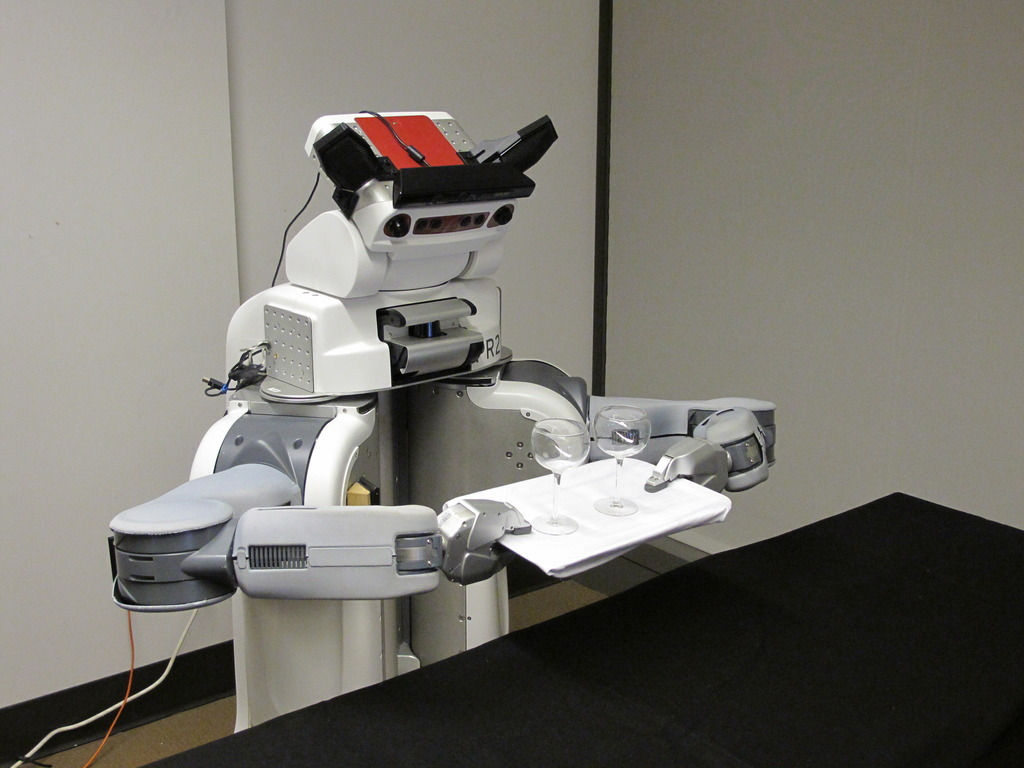
\includegraphics[width=0.7\textwidth]{dual-000.jpg}
\caption{The PR2 robot holding a tray with glasses}
\label{fig:PR2 with glasses}
\end{figure}



\section{Introduction and Related Work}
% no \IEEEPARstart
This report is  a review of the article \emph{Search-based Planning for Dual-arm Manipulation with Upright Orientation Constraints} by \emph{Benjamin Cohen, Sachin Chitta} and \emph{Maxim Likhachev}, published at \emph{IEEE Int. Conference on Robotics and Automation} in 2012, see [24].\\
In human environments it is sometimes hard or even impossible to deal with an object using only one hand. For example, carying any big objects such as big boxes or objects that require correct orientation is space such as trays with glasses etc. is much easier with the use of both hands instead of just using one. This is why these tasks are often performed with usage of both hands by human. This is the motivation for performing such tasks with two arms by a general mobile robot.\\


As was mentioned before, sometimes it is necessary to hold and carry objects with constraints on their orientation. For example, carying a tray with food or glasses requires naturally an upright orientation constraint at each moment of the movement. In real life these tasks are usually performed by humans in cluttered environments e.g. moving a tray through an environment full of obstacles. These tasks involve fast and efficient planning of actions, while retaining the upright orientation constraint. This is exactly what is addressed in this paper.\\
The robot that was used for this task is the PR2 robot. In Figure 1 it is shown holding a tray with two wine glasses on it. For this task the robot has to maintain the upright orientation of the tray throughout the sequence of arm motions. Navigating in cluttered environments with a tray is a hard task, that involves many different parts such as planning the collision-free apth through the environment while preserving the upright orientation constraint of the tray. The authors of the paper focus only on the dual-arm manipulations part.\\
Motion planning for dual-arm manipulations is addressed as a graph search problem in this paper. The graph is constructed in action space and heuristic search such as A* [8] and its variants is used to find the optimal sollution to the problem.\\
In recent years manipulating objects in human environments gained a lot of interest ([19], [18], [7], [1], [11], [2], [22]). The works [4],[5] and [6] show successfull usage of A*-like search algorithms on graphs with correspondence to motion planning including single arm manipulations and other mobile manipulation tasks. These algorithms have advantages such as good cost optimmization and strong theoretical guarantees on completeness and optimality or bounds on the sub-optimality of the sollution [17]. Another benefit of graph-based techniques is their consintensy. That makes the robot behave predictably given the same start and goal poses which is very important in human environments as people are able to predict the robot's actions better.\\
On the other hand, the gurantees of optimality as well as consistensy are with respect to the graph which is used to represent the planning problem, so they are discretization of state and action space dependent.\\
However the A*-like algorithms were never used for dual-arm manipulations before. Recently, as interest in dual-arm manipulations has rised, a couple of dual-arm platforms became available, e.g. the robot used in this paper - PR2 [3] (Fig. 1), Intel HERB Personal Robot [22], ARMAR III [23] and Justin [2]. Dual-Arm manipulation was already used for tasks like cart-pushing [21], towel folding [16] and the manipulation of small kitchen objects [23]. Usually, unlike the approach chosen by the authors of this paper, randomized motion planners were chosen to perform on above mentioned tasks. For example, in [23], randomized motion planners were used for planning re-grasping actions and dual-arm motion plans for a humanoid robot with two arms. Impressive results for combined grasping and motion planning were achieved by interleaving the efficient computation of inverse kinematics using a pre-computed reachability map with the motion planning itself. In [10], an assembly task was executed with two arms using combined task and motion planning. Online manipulation planning for objects moving on a conveyer belt was carried out in [14] for two 2-DOF arms. In [12], one of the first approaches to planning for dual-arm manipulation was presented using a randomized planner. Multi-arm manipulation planning, including the planning of transfer paths and grasp and ungrasp motions for manipulating an object using multiple arms was presented in [13]. The results of this approach were demonstrated on a simulated system manipulating a simple object using 3 arms.\\
Randomized planners for dual-arm manipulation tasks are a popular choise popular because of their speed and ease of implementation. However, plans generated by such planners require frequent post-processing, e.g. using a short- cutting approach [9], before they can be executed on a robot. In addition, due to the random nature of the planners, the generated paths are also inconsistent across runs, i.e. paths planned for the same environment for similar start and goal positions are likely to be very different. Search-based planning addresses this issue providing consistency between runs and reasonable cost minimization.\\
The authors of this paper present a graph-based A* search approach for dual-arm manipulation that is based on two key components: the representation of the state space and a novel heuristic. 
The representation of the state space is chosen so that it reduces the dimentionality of the problem and thus makes it easier to ba handeled via search-based techniques. It also helps dealing with discretization artifacts that authors of the paper have experienced in their former work [6].
The heuristic function is chosen in the way that it exploits the upright orientation constraint of the object. This provides additional information for motions in a cluttered environments.\\
This paper will focus mostly on these two concepts.

\section{The PR2 Robot REWRIGHT}
The hardware platform that was used for experiments by the authors of the paper was the PR2 mobile manipulation robot (Fig. 1). The PR2 robot is a two-armed robot with an omni-directional base and a variety of sensors mounted on a sensor head. Each arm has 7 degrees of freedom and thus has a redundant degree of freedom. In this paper, the redundancy is exploited by developing a custom inverse kinematics solution for the arm that is parameterized by one of the joint angles. The joint angle we choose is the upper arm roll joint shown in Fig. 3(b). The joint limits on the robot’s joints are also taken into account by the kinematics solver. Thus, given the end-effector pose and a value for the free parameter, we can deterministically compute the corresponding inverse kinematics solution for this pose. In general, because of joint limits, we tend to find only a single solution (if it exists) for a given end-effector pose and free angle parameter. If a solution does not exist, it is possible to step through the full range of motion of the redundant joint to search for an inverse kinematics solution.

\section{Motion Planning Algorithm (under construction)}
The morion plasnnin algorithms described in this paper is based on constructing and serching a motion-primitive based graph [5] using pre-defined and runtime-generated motion primitives. The graph search is supposed to find a path from start configuration of the robot to its goal configuration (location and orientation).\\
The algorithm consists of these four parts:\\
 - Graph constuction;\\
 - Cost function;\\
 - Heuristic;\\
 - Search;
\subsection{Graph Construction}
In the previous work, the authors of the paper  represented the configuration space of the arm in joint space [5]. This results in a graph with 7 dimentions for the robot arm with 7 DoF. This means if the graph for current problem would be constructed in the same manner this would result in a 14 dimentional statespace. This number can be reduced using the object constaint as follows.\\
The notation $G=(S,E)$ will be used further to denote the graph $G$ that is being constructed, where $S$ denotes the set of states of the graph and $E$ - the set of transitions between states. The states set $S$ is the set of possible 3 DoF poses of the object coupled with the redundant joint angles. That means that that each state $s$ is defined as a 6-tuple, $(x,y,z,\theta_{yaw}, \theta_1, \theta_2)$. Here $(x,y,z)$ denote the global position of the center of the object, $\theta_{yaw}$ is the object's global yaw angle and $\theta_1, \theta_2$ are the joint positions of the redundant joint in the right and left arm of the robot respectively (Figure 2).\\
The transitions in $E$ are a set of feasible motions primitives, which is defined as a vector of velocities of the object and the two redundant joint velocities. As pre-allocation is infiesable for a 6 dimentional graph it is constructed dynamically by the graph search as it expands states. The set of motion primitives is shown in Figure 3. It consists of the 26 translational motions that just move the object one cell, two motions that rotate each free angle in both directions.\\
Before a successor of state $s$, state $s'$ can be added to the graph it must be checked for feasibility by checking that joint configurations for both arms exist within the joint limits and are collision free. The authors use an inverse kinematics solver to compute joint configurations for each arm that satisfy the state's coordinates. The solver may fail if the found sollution violates the joint limits of the arms. If this is not the case, then the arm configurations are forward simulated and checked for collisions with each other, obstacles in the environment and for collisions of the object with environment.\\
If the inverse kinematics solver fails for one or both of the arms, then instead of rejecting the motion the authors search over the redundant angles of the arms of the robot for possible sollutions. If the sollution exists, then an adaptive motion primitive [6] is generated. It is also called "a primitive generated at runtime". That is, the motion primitive that was rejected is duplicated, but with different values of $ \theta_1 $ or $ \theta_2 $ or both.\\
Authors of the paper also note that while they are using a fairly simple set of motion primitives a more complex one can be used aswell. This would result in smoother path at the expense of planning time.\\
In previous works the authors of this paper used joint space representation [6] as task space representation. The appoach provided in this work is advantageous over the old one because now the path length is being optimized in the position space of the object, which allows for multiple joints to be moved at the same time. Previously the set of primitives limited the trajectory to move only one joint at a time. The new approach also gives the opportunity for the heuristic function to be easier for the search to follow and more informative.
\subsection{Cost Function}
The cost function is designed to minimize the path length of the end effector while maximizing the distance between the manipulator and the nearby obstacles along the path. That is, the cost of any transition in the graph is designed as follows: $c(s,s')=c_{cell}(s')+c_{action}(s,s')$, where $c_{cell}$ is a cost applied to the cells that are situated near the obstacles, to discourage creating the path through them, $c_{action}$ is the cost of the motion primitive. In the provided work $c_{action}$ was determined by the user and $c_{cell}$ was defined so that a cell is twice as expensive as normal cell if the configuration of the arm is within 20 cm of the obstacle and five times the cost of normal cell when the distance is less then 10 cm. It is alsp possible to add the third summant, which would penalize large changes in any of the joint angles.\\
the alternative cost functions was also defined in the paper. It penalizes the execution time of planned trajectory. The planner is configured with desired joint velosities. The cost is then computed as the longest joint motion time multiplied by desired cost per second.\\
It is stated, that usually both approaches tend to create alike trajectories. However this approach was not used further in the paper.\\
\subsection{Heuristic}
As the algorithm that is used inthe paper is heuristic-based it is needed to specify admissable and consistent heuristic function. This function has to efficiently avoid obstacles as the robot is intended to run in cluttered environments. Earlier the authors of the paper used a 3D Dijkstra algorithm search to compute the cost of the least-cost path from the position of the inner sphere of the object at a given state to the object pose at the goal state. However, in this paper, as the upper orientation constraint is given, instead of modelling the object using the inner sphere, an inner cyllinder is used, as the object is constrained from pitching and rolling. This cyllinder is situated in the geometric center of the object and its radius is the radius of the inner circle of the object.\\
The heuristic function is computed as follows: the obstacles are inflated by the radius of inner circle of the object for each $xy$ plane by iterating through $z$-axis of the grid. Then on each call of heuristic function $h(x,y,z)$, we check if cells $(x,y,z),(x,y,z+1),...,(x,y,z+n)$ are collision free. Detailed example is presented on Figure 4.\\
It is also stated that using the outer circle may also be used, which may appear to be much more informative, though this results in sacrifising the completeness of the planner.\\
The heuristic for a given state is computed when needed, unlike the approach the authors of the paper used in [6], where the heuristic was precomputed for the entire workspace before planning started. This took 0.6 seconds. Instead, now initially the Dijkstra search is run until it expands the start state. Then if the search ever encounters a state which has not yet been added to the Dijkstra search tree, the Dijkstra search until the state of interest is expanded would be resumed. This way expanding all of the states in the environment is avoided.\\
\subsection{Search}
Any standard graph search algorithm can be used to search the graph G that is constructed. Given the complexity of the graph, however, optimal graph search algorithms such as A* [8] are infeasible to use. Instead we chose an anytime version of A* - Anytime Repairing A* (ARA*) [15].This algorithm generates an initial, possibly suboptimal solution quickly and then concentrates on improving this solution while deliberation time allows. The algorithm guarantees completeness for a given graph G and provides a bound $\epsilon$ on the suboptimality of the solution at any point of time during the search. ARA* speeds up the typical A* search by inflating the heuristic values by a desired inflation factor, $\epsilon$. An $\epsilon$ greater than 1.0 will produce a solution guaranteed to cost no more than $\epsilon$ times the cost of an optimal solution in the graph.
\section{Experimental Results}
The authors of the paper manually picked  start and goal poses for the object, by generating inverse kinematics solutions corresponding to them and checking that sollutions are collision free. In total twelve experiments were taken, all inspired by practical manipulation scenarios in four different cluttered environments with five different objects (Figure 5). The actual object used are shown in Figure 6. All twelve experiments were first run in simulation and then on real robot. Table 1 shows the results of simulated experiments. In all of the runs the planner was initialized with an $\epsilon$ = 100 and was given 15.0 seconds to generate a more optimal solution if time permitted. The $\epsilon$ of the final solution found is listed in the third column. The planning times include the time it takes to compute the heuristic. The resolution of the object's pose is 2cm for the position and 5 for the yaw of the object as well as 2 for both of the redundant joints. All of the tests require that the planner computes a path to a 4-DoF pose constraint for the object with a tolerance of 5 in the final yaw of the object and a 2cm tolerance in the position of the object. The redundant joint angles do not need to reach the goal location. The set of 32 motion primitives shown in Figure 3 was used.\\
Table II shows the results of the same set of experiments but using the radius of the outer circle to compute the heuristic.\\







\end{document}
